\documentclass{logo-cv}
% ======================== Plain version =================================== %
\newCJKfontfamily\mynamefont{Source Han Serif CN}

% ======================== University version ============================== %
\definecolor{customcolor}{RGB}{71,96,169}
\newcommand{\aLogo}{
\includegraphics[width=0.18\textwidth]{images/logo-white.pdf}}
\newcommand{\bLogo}{
\includegraphics[width=0.75\textwidth]{images/badge-blue.pdf}}
\newcommand{\school}{兰州大学 | Lanzhou University}
\newcommand{\contact}{\textcolor{white}{\textbf{求职方向：AI推理部署与异构计算}}}
\setlength{\headheight}{17pt}


\begin{document}
\section{个人信息与教育背景}
\begin{minipage}{0.14\textwidth}
    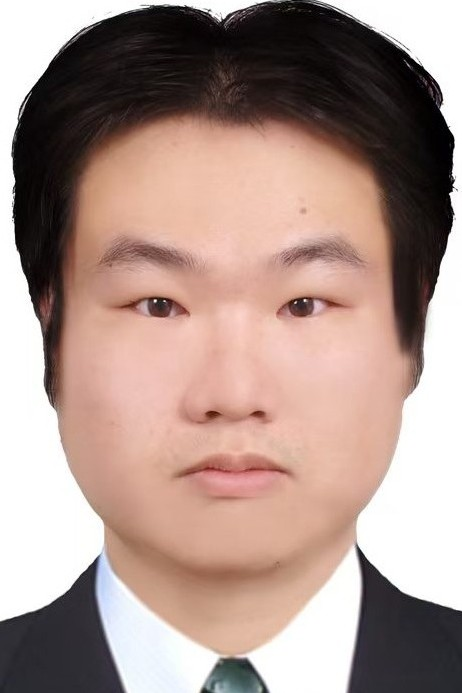
\includegraphics[height=0.7\textwidth]{images/Me_s.jpg}
\end{minipage}
\begin{minipage}{0.28\textwidth}
        \begin{tabular}{ll}
        \textbf{姓名} & {\mynamefont 许忞欢}         \\
        \textbf{电话} & 19525029181     \\
        \textbf{邮箱} & xumh2001@gmail.com \\
        \textbf{籍贯} & 江苏无锡 \\
        \textbf{方向} & AI推理部署、异构计算  \\
        \end{tabular}
\end{minipage}
\hfill
\raisebox{-0.085\textwidth}[0pt][0pt]{\textcolor{customcolor}{\rule{0.5pt}{0.17\textwidth}}}
\hfill
\begin{minipage}{0.49\textwidth}
\begin{cSubsection}{兰州大学（985工程）}{2024.9 - 至今}{信息与通信工程（前5\%）}{硕士}
\end{cSubsection}
\begin{cSubsection}{兰州大学（985工程）}{2020.9 - 2024.6}{电子信息省级基地班（\emph{前20\%，免试攻读硕士}）}{学士}
\end{cSubsection}
\end{minipage}

\section{专业技能}
\begin{itemize}
    \item \textbf{编程与工程} \hfill 熟练使用C/C++、Python及MATLAB，具备Linux环境开发、故障排查与Git代码管理能力
    \item \textbf{异构部署} \hfill 具备NVIDIA Jetson、GPU、FPGA及Zynq SoC实践，掌握TensorRT部署及PCIe/XDMA数据链路
    \item \textbf{AI算法} \hfill 熟悉YOLO、强化学习、逆强化学习、Transformer及神经网络训练流程，具备模型部署与调度经验
    \item \textbf{软硬件协同} \hfill 熟悉Vivado、Vitis、STM32和Qt，能够开展算法验证、数据预处理、系统集成及性能分析
    \item \textbf{基础能力} \hfill 英语CET-6；具备技术调研、方案验证和技术文档撰写能力
\end{itemize}

\section{科研成果}
\begin{itemize}
    \item 研究方向：非线性系统的鲁棒控制、逆强化学习与智能控制算法
    \item 论文《Inverse Reinforcement Q-Learning for Stochastic LQR of Nonlinear Systems》：IEEE TIE一审大修
\end{itemize}

\section{项目工作}
\begin{itemize}
    \item 横向项目：智能训练与开发平台研究（中国航空工业集团公司雷华电子技术研究所） \hfill 2026.04 - 至今
    \begin{itemize}
        \item \textbf{项目简介}：面向雷达探测、电子干扰、侦察识别和通信场景，建设“云平台—边缘计算—数字信号端”协同的智能训练与开发平台，实现高带宽、低时延、高并发信号处理。
        \item \textbf{项目贡献}：负责边缘计算节点与FPGA之间基于XDMA的高速稳定数据交换；参与云端模型部署与调度管理，并基于容器技术开发集群主控及存储节点，打通模型从云端到异构硬件节点的部署链路。
    \end{itemize}
    \item 横向项目：通用辐射效应测试平台研制（兰州空间技术物理研究所） \hfill 2025.10 - 至今
    \begin{itemize}
        \item \textbf{项目简介}：通过高速ADC采样对特定信号进行实时分析，并利用FPGA完成低时延处理与反馈，实现电子设备辐射效应测试。
        \item \textbf{项目贡献}：负责Zynq-7000 SoC端开发，完成PL与PS之间的高速数据传输，以及PL端去直流预处理和脉冲检测；围绕吞吐、时延与处理正确性开展软硬件联调。
    \end{itemize}
    \item 保密项目：《xxxx》 \hfill 2023.09 - 2025.10
    \begin{itemize}
        \item \textbf{项目简介}：xxxx
        \item \textbf{项目贡献}：作为主要软件开发者，完成FPGA与GPU异构平台相关功能开发、系统集成及测试，积累了算法软硬件协同落地经验。
    \end{itemize}
    \item 混沌加密图像传输 \hfill 2023.09 - 2025.10
    \begin{itemize}
        \item \textbf{项目简介}：面向FPGA与NVIDIA Jetson之间的图像加密及高速传输需求，开发异构平台数据处理链路。
        \item \textbf{项目贡献}：针对PCIe接口及加密算法数据格式要求，设计彩色图像压缩、重排、int32封装与还原流程，并基于C++/OpenCV实现数据预处理和传输，完成端到端功能验证。
        \item \textbf{模型部署}：在NVIDIA Jetson平台上使用TensorRT部署YOLO模型，完成模型推理与运行验证。
    \end{itemize}
    \item 国家自然科学基金：《复杂环境下机器人运动控制的模仿学习技术》 \hfill 2023.01 - 至今
    \begin{itemize}
        \item \textbf{项目简介}：面向复杂环境下的机器人运动控制，研究模仿学习、逆强化学习及模型控制算法，并完成机器人控制平台设计。
        \item \textbf{项目贡献}：基于Qt开发上位机与数据处理模块，完成手持控制器、嵌入式软件及多传感器集成；研究履带车、机械臂与机械手运动学及控制策略，并利用Leap Motion实现手势识别。
    \end{itemize}
    \item 甘肃省重点研发计划：《机器人抗干扰高精度模型预测控制》 \hfill 2025.02 - 至今
    \begin{itemize}
        \item \textbf{项目简介}：面向空间灵巧手，开展非线性高精度建模、强化学习抗干扰控制及Transformer多任务学习研究。
        \item \textbf{项目贡献}：针对复杂环境中的状态测量误差与对抗噪声，基于状态对抗马尔可夫决策过程改造深度强化学习算法；结合最强对抗噪声搜索与鲁棒策略正则化，构建鲁棒强化模型预测控制方案并开展算法验证。
    \end{itemize}
\end{itemize}

\section{本科校内工作}
\begin{itemize}
    \item 国家级大学生创新创业训练计划《基于Python的〈信号与系统〉仿真平台设计与实现》 \hfill 2022.5 - 2023.5
    \item 计算机软件著作权《基于Python的〈信号与系统〉连续信号仿真平台设计与实现V1.0》 \hfill 2023.4
\end{itemize}

\section{学业荣誉}
\begin{itemize}
    \item 兰州大学优秀学生一等（2020）、二等（2021--2022）奖学金 \hfill 2020.9 - 2022.12
    \item 兰州大学优秀研究生一等（2025）、二等（2024）奖学金 \hfill 2024.9 - 2025.12
\end{itemize}

\section{自我评价}
具备AI算法、嵌入式开发与异构计算交叉背景，能够使用C/C++、Python完成算法实现、数据处理和系统联调；拥有NVIDIA Jetson、GPU、FPGA及Zynq SoC平台实践，理解模型部署中数据链路、计算资源与实时性之间的权衡。具备独立技术调研、方案验证和问题定位能力，能够面向实际需求推进算法在软硬件平台上的工程落地。
\end{document}
